\chapter{Slope Limiter Methods}
%%%%%%%%%%%%%%%%%%%%%%%%%%%%%%%%%%%%%%%%%%%%%%%%%%%%%%%
\section{Method Recap}
In the Chapter 5, we looked at the Upwind Euler, Centered Leapfrog and Lax-Wendroff methods. Setting aside the Centered Leapfrog as it is the most inaccurate for evolving a step function, we now look at the Upwind, Lax-Wendroff and Lax-Friedrich instead. By looking at Figure \ref{fig:lw_lf_ue} we can see that the Lax-Wendroff performs the best, although marginally, against the other two methods on the Gaussian pulse but the worst at the heaviside step function. The Upwind Euler, however, performs best on the heaviside step function but none of these methods are able to adequately evolve the heaviside step without some form of sloping or erratic behaviour at the shock points. Therefore we need a method which adequately evolves both smooth, differentiable functions and functions with sharp points or steps, these are known as High-Resolution Methods or Slope/Flux Limiter Methods.
\begin{figure}[H]
  \centering
  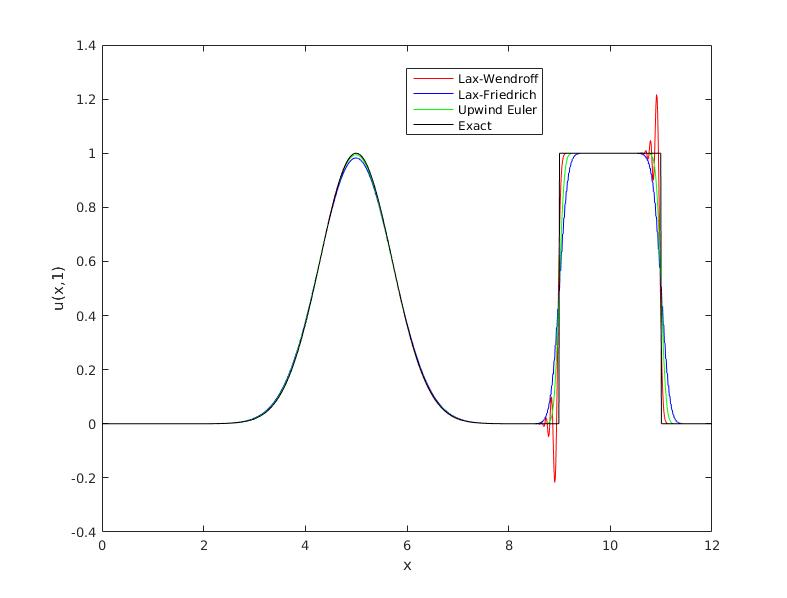
\includegraphics[width=0.7\textwidth]{Images/7_lw_lf_ue.jpg}
  \caption{Comparison of Lax-Wendroff, Lax-Friedrich and Upwind Euler methods}\label{fig:lw_lf_ue}
\end{figure}
%%%%%%%%%%%%%%%%%%%%%%%%%%%%%%%%%%%%%%%%%%%%%%%%%%%%%%%
\section{Slope Limiter Methods}
Slope Limiter Methods (SLMs) are a special form of Piecewise-Linear functions which in turn are a more complex form of a Reconstruction Method (Section \ref{sec:recon}). All SLMs take the form of
\begin{equation}\label{eq:slm}
  v^{n+1}_j = v^n_j + \frac{k}{h}(f(v^n_{j+1}) - f(v^n_{j-1})) + \frac{1}{2}(h-ck)(\sigma^n_j - \sigma^n_{j-1})
\end{equation}
They differ in how they choose $\sigma^n_j$ to be used to calculate the slope of the cell. There are three different potential forms of $\sigma$, namely
\begin{align*}
  \sigma_{us} &= \frac{v_j     - v_{j-1}}{h} \text{ Upwind Slope}  \\
  \sigma_{ds} &= \frac{v_{j+1} - v_j}{h} \text{ Downwind Slope} \\
  \sigma_{cs} &= \frac{v_{j+1} - v_{j-1}}{2h} \text{ Centered Slope}
\end{align*}
%------------------------------------------------------
\subsection{Minmod}
Minmod is the simplest of these methods, using the minmod function as follows
\begin{align*}
  minmod(a,b)   &= a &if |a| < |b|\\
                &= b &if |b| < |a|\\
                &= 0 &if ab < 0
\end{align*}
to determine the value of $\sigma^n_j$. It does this by setting the value as
\begin{equation*}
  \sigma^n_j = \text{ minmod}(\sigma_{us},\sigma_{ds})
\end{equation*}
%------------------------------------------------------
\subsection{Superbee}
The Superbee works by finding a maxmod (similar to a minmod) of two values of which the minimum has been found.
\begin{gather*}
  \sigma^n_j = \text{ maxmod}(\sigma^1,\sigma^2) \\
  \text{where:} \quad \sigma^1 = \text{ minmod}(\sigma_{ds},2\sigma_{us}) \quad \text{and} \quad \sigma^2 = \text{ minmod}(2\sigma_{ds},\sigma_{us})
\end{gather*}
It biases the weighings in such a way that even if one of the gradients is much larger than the other, the resulting gradient isn't too biased to the smaller gradient.
%------------------------------------------------------
\subsection{MC Mod}
The MC Mod method uses the minmod of all three gradient measures to determine the next value, it biases the value of the central slope as it is seen as the average of the three values.
\begin{equation*}
  \sigma^n_j = \text{ minmod}(\sigma_{cs},2\sigma_{us},2\sigma_{ds})
\end{equation*}
\subsection{Analysis}
By using these three methods on the same function as Figure \ref{fig:lw_lf_ue}, we can see in Figure \ref{fig:mm_sb_mc} that these methods provide a high accuracy for both the Gaussian and the heaviside step functions and have a steeper step than that of the Upwind Euler.
\begin{figure}[H]
  \centering
  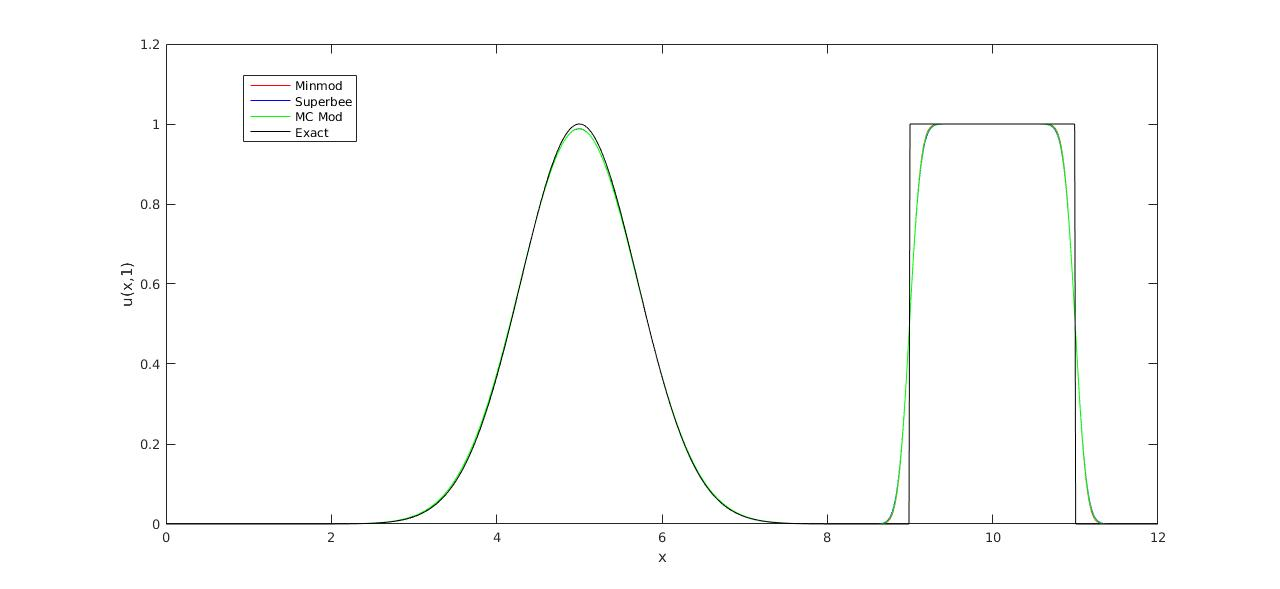
\includegraphics[width=0.7\textwidth]{Images/7_mm_sb_mc.jpg}
  \caption{Comparison of Minmod, Superbee and MC Mod methods}\label{fig:mm_sb_mc}
\end{figure}